\documentclass[border=6pt]{standalone}
\usepackage{tikz}
\usetikzlibrary{arrows.meta}
\begin{document}
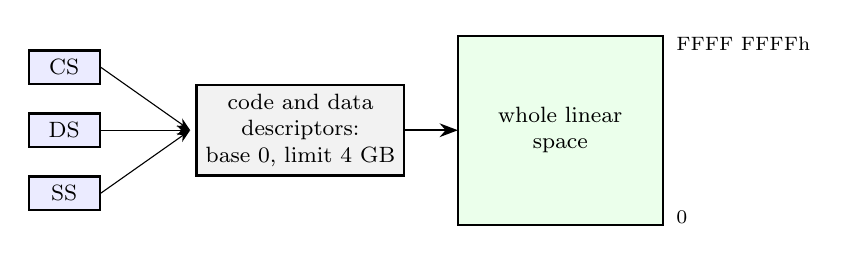
\begin{tikzpicture}[>=Stealth,font=\small]
\foreach \r/\y in {CS/0.8,DS/0,SS/-0.8} { \node[draw,thick,fill=blue!8,minimum width=0.9cm,font=\footnotesize] (\r) at (0,\y) {\r}; \draw[->] (\r.east) -- (1.6,0); }
\node[draw,thick,fill=gray!10,align=center,font=\footnotesize] (d) at (3.0,0) {code and data\\descriptors:\\base 0, limit 4 GB};
\draw[->,thick] (d.east) -- (5.0,0);
\draw[thick,fill=green!8] (5.0,1.2) rectangle (7.6,-1.2);
\node[font=\footnotesize,align=center] at (6.3,0) {whole linear\\space};
\node[font=\scriptsize,anchor=west] at (7.65,1.1) {FFFF FFFFh};
\node[font=\scriptsize,anchor=west] at (7.65,-1.1) {0};
\end{tikzpicture}
\end{document}
